\begin{savequote}[8cm]
\textlatin{Neque porro quisquam est qui dolorem ipsum quia dolor sit amet, consectetur, adipisci velit...}

There is no one who loves pain itself, who seeks after it and wants to have it, simply because it is pain...
  \qauthor{--- Cicero's \textit{de Finibus Bonorum et Malorum}}
\end{savequote}

\chapter{\label{ch:4-spk}Single Particle Kinematics Improvement} 

\minitoc
   The granular structure of SFGD brings many improvements to single-particle kinematics measurement. 
   This is especially important for hadrons, as they tend to have shorter tracks and hence poorer momentum resolution compared to muons. 
   Two of the most common product hadrons from neutrino-nucleus interaction are protons and pions. 
   The default particle identification and momentum reconstruction have been developed by colleagues at T2K using the Boosted Decision Tree (BDT) algorithm. The BDT algorithm has good performance, but it is still lacking in some aspects.
   For instance, as it uses only single-track information, it cannot effectively distinguish between pions and muons. 
   It could reconstruct proton momentum with an excellent resolution of about $3.5\%$, but it is insufficient for TKI analysis, which is highly sensitive to hadron kinematics. 
   To address these gaps, I have developed and implemented new techniques for both hadrons. 
   For pions, I have invented the pion trackless reconstruction, a novel technique to reconstruct pions without requiring the presence of a reconstructed track, thereby lowering the detection threshold and significantly increasing reconstruction efficiency for low-momentum pions. 
   As for protons, I have adapted the Elastically Scattered and Contained (ESC) protons technique~\cite{Lu:2016mjf} first implemented in MINERvA to create an ESC proton selection in SFGD, leading to a proton sample with excellent momentum resolution. 
   
    %------------------- pion TL ----------------%
    \subsection{Pion Trackless Reconstruction}
       In SFGD, when particles pass through the detector, they deposit energy and emit scintillation light, which would be captured by the three optical fibres and the electronics connected to the end of the fibres, 
       The signal from each cube constitutes a "Hit". 
       All Hits are fed into the existing tracking algorithm, which tries to find a track pattern through the Hits. 
       If such a track is possible, the Hits along the track are grouped into "Nodes" consistently as points along the track. 
       Particle identification and momentum reconstruction are then performed on these reconstructed tracks. 
       It is clear from this track reconstruction process that, for a track to be reconstructed, it has to be long enough, i.e. containing at least $3$ nodes, corresponding to about $30\textrm{mm}$. 
       Hence, low-momentum particles, which travel only a short distance, could not be reconstructed at all. 
       When these low-momentum pions are not reconstructed, these $\ccopi$ events would then be misidentified as $\cczpi$ events, both decreasing the signal for the $\ccopi$ samples and increasing the background for the $\cczpi$ sample. 
       Thus, it would be highly beneficial if we could reconstruct these pions, and the pion trackless reconstruction technique I develop can address this gap perfectly. 

       \subsubsection{Working Principles}
         The trackless technique is an extension and sophistication of previous methods. 
         It was first tried in MINER$\nu$A\cite{MINERVAPOSTER} and in the Fine Grain Detectors of ND280\cite{T2KPOSTER}. 
         In the former, at least a reconstructed cluster is required to be identified as a pion candidate. 
         The latter indeed contains a prototype of the trackless reconstruction, but it is mixed with other pion reconstruction methods and its potential is not fully explored. 
    
         There are two key points of this reconstruction technique based on the pion decay chain, $\pi \rightarrow \mu \rightarrow e$.
         Firstly, the delayed signal of the grandchild, the Michel Electron (ME), is much longer than the time scale of other processes, such as $\piz$ decay.
         Hence, the presence of the primary pion can be inferred by the presence of a delayed signal in the SFGD.
         Secondly, the pion decay, $\pi \rightarrow \mu + \nu$, is a two-body process, the kinematics of the daughters can be completely determined by energy-momentum conservation, 
         When a pion decays at rest, the daughter muon will only move about $0.12~\textrm{cm}$. Hence, the starting point of the ME is a good estimation of the ending point of the pion.
         The pion momentum can then be reconstructed by range based on the distance between the primary neutrino interaction vertex and the ME starting point. 
         A relation between the pion momentum, via its kinetic energy, and its range is obtained from an empirical fit on particle gun simulation, as shown in shown in \figref{fig:fit}.
        
           \begin{figure}[h]
              \centering
              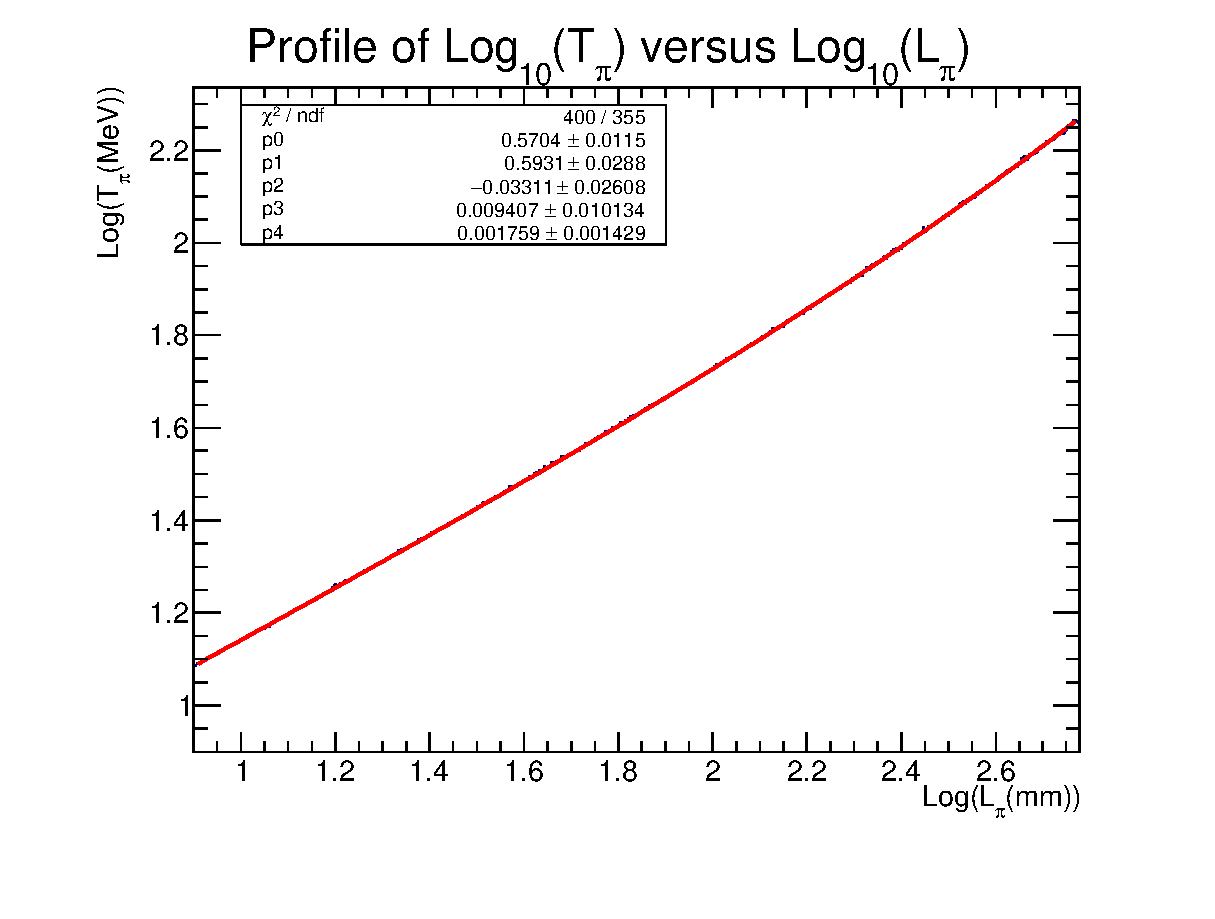
\includegraphics[width=0.5\textwidth]{fig/hplog_KE_len_with_p_log10_pol4_60260_pf0.eps} 
              \caption{A degree 4 polynomial fit of $\log_{10}{T_\pi}$ against $\log_{10}{L_\pi}$, where $T_\pi$ and $L_\pi$ are the kinetic energy and the range of the pion respectively. The $p_i$'s are the corresponding coefficients of the term of order $i$. The fit is satisfactory considering the close to 1 $\chi^2/ndf$ value. }
              \label{fig:fit}
           \end{figure}

        \subsubsection{Implementation}
            The pion trackless reconstruction is part of my $\numuccopi$ selection, which is based on the existing $\numucc$-inclusive selection. Hence, it is best to elaborate the trackless technique in the context of the $\numuccopi$ selection. 
        
            The $\numucc$-inclusive selection has identified the primary vertex position and the primary muon, which already provides the trackless reconstruction with a good approximation of the pion starting point. The following steps are implemented to identify the suitable ME and reconstruct the pion momentum in the $\numuccopi$ selection. 

            \begin{itemize}
                \item Step 0 - \textbf{$\numucc$-inclusive selection.}
                \item Step 1 - \textbf{Find suitable ME candidates.} 
                \item Step 2 - \textbf{One trackless pion cut.}
                \item Step 3 - \textbf{Kink cut.}
                \item Step 4 - \textbf{Background reduction.}
            \end{itemize}
        
            \textbf{Find suitable ME candidates.} - Loop through all delayed reconstructed objects that have more than 1 hit, if it is $30.0~\textrm{ns}$ after the primary vertex time, save it as a potential ME candidate. 
            However, it is common that the ME could trigger a shower, leading to more delayed reconstructed objects. 
            To distinguish the ME from these secondary delayed objects, a technique called the "prompt energy" was used by MINERvA~\cite{Zhang2016}. 
            Prompt energy is the energy deposited by the short muon and the short pion. 
            Even though these particles might have too low energy to leave a reconstruct-able track, they would still deposit energy, which is much early than the onset of ME. 
            Hence, looping through the cubes $30.0~\textrm{mm}$ around the two ends of an ME candidate to observe if there is energy deposited $30.0~\textrm{ns}$ before identifying the proper ME candidate. 
            Moreover, if the primary muon is contained in SFGD, it would also decay to give an ME, which is indistinguishable from a pion ME by just looking at the time delay. 
            Hence, an additional check is added to exclude ME candidates near the end of the identified primary muon. 
        
            \textbf{One trackless pion cut} - Select events that have one and only one proper ME candidate.
        
            \textbf{Kink cut} - As the trackless reconstruction does not require the ME to be near a primary track, it cannot distinguish pions travelling straight from the primary interaction until decaying at rest from those that have undergone a deflection and then decayed at rest. 
            Events with a deflected pion should be rejected as the momentum-by-range reconstruction works only for particles without secondary interaction. 
            Hence, events with an ME connected to any non-primary tracks would be rejected.
        
            \textbf{Background reduction} - Several background reduction steps are implemented, for example, an existing $\pi^0$ rejection developed by Colleagues at T2K.
        
            For the events passing all the selection steps, the presence of a primary pion is implied by the existence of a proper ME candidate, and its momentum is reconstructed by range. 
            
        
        \subsubsection{Results}
            The results of the $\numuccopi$ selection using the trackless pion technique are summarised in Fig.~\ref{fig:piTLres}.
           As shown in Fig,~\ref{fig:ppi-stack}, the trackless selection has achieved the set goal - reconstructing low momentum pions. 
           There are a considerable number of events with a pion below $100~\mevc$, which correspond to a track of about $50~\textrm{mm}$. 
           Moreover, pions below $80~\mevc$ have also been reconstructed, which travels about $30~\textrm{mm}$ and cannot be reconstructed as a track. 
           Furthermore, the momentum-by-range calculation has achieved an excellent resolution at about $2\%$, as shown in $\ref{fig:ppi-res}$.
           More encouragingly, the overall efficiencies are still relatively high. 
           The step-by-step efficiencies with respect to each step is shown in Fig.~\ref{fig:tl-accum-eff}. 
           The signal definition used in the calculation is to have one true muon that has travelled to the vertical TPC and one true pion that is contained in SFGD. 
           Steps 1 to 7 are the $\numucc$-inclusive selection. 
           The large drop in efficiency in Step 8 is expected as it requires exactly one pion reconstructed tracklessly. 
           All pions undergoing secondary interactions except deflection cannot be reconstructed via this method. 
           Hence, the relative efficiency of $0.37/0.66\approx56\%$ is considerably high. 
           The further significant drop in efficiency comes with the next step, the kink cut, which is a reasonable as a considerable portion of pions undergo deflection. 
           The subsequent drops are graduate cuts to remove backgrounds, which leads to a high purity of $\numuccopi$ as shown in Fig.~\ref{fig:ppi-stack}.

           \begin{figure}[t]
               \centering
               \begin{subfigure}{0.3\textwidth}
                    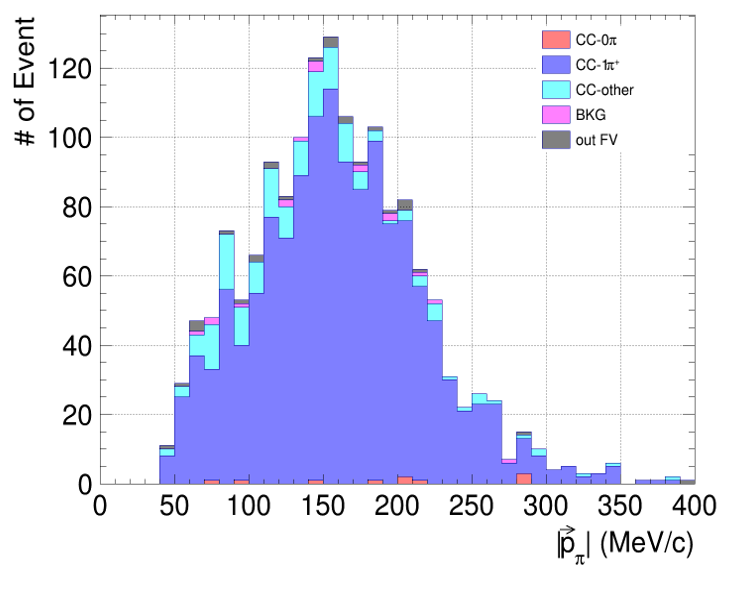
\includegraphics[width=\textwidth]{fig/ppi_stack.png}
                    \caption{Momentum distribution.}
                    \label{fig:ppi-stack}
               \end{subfigure}
               \begin{subfigure}{0.3\textwidth}
                    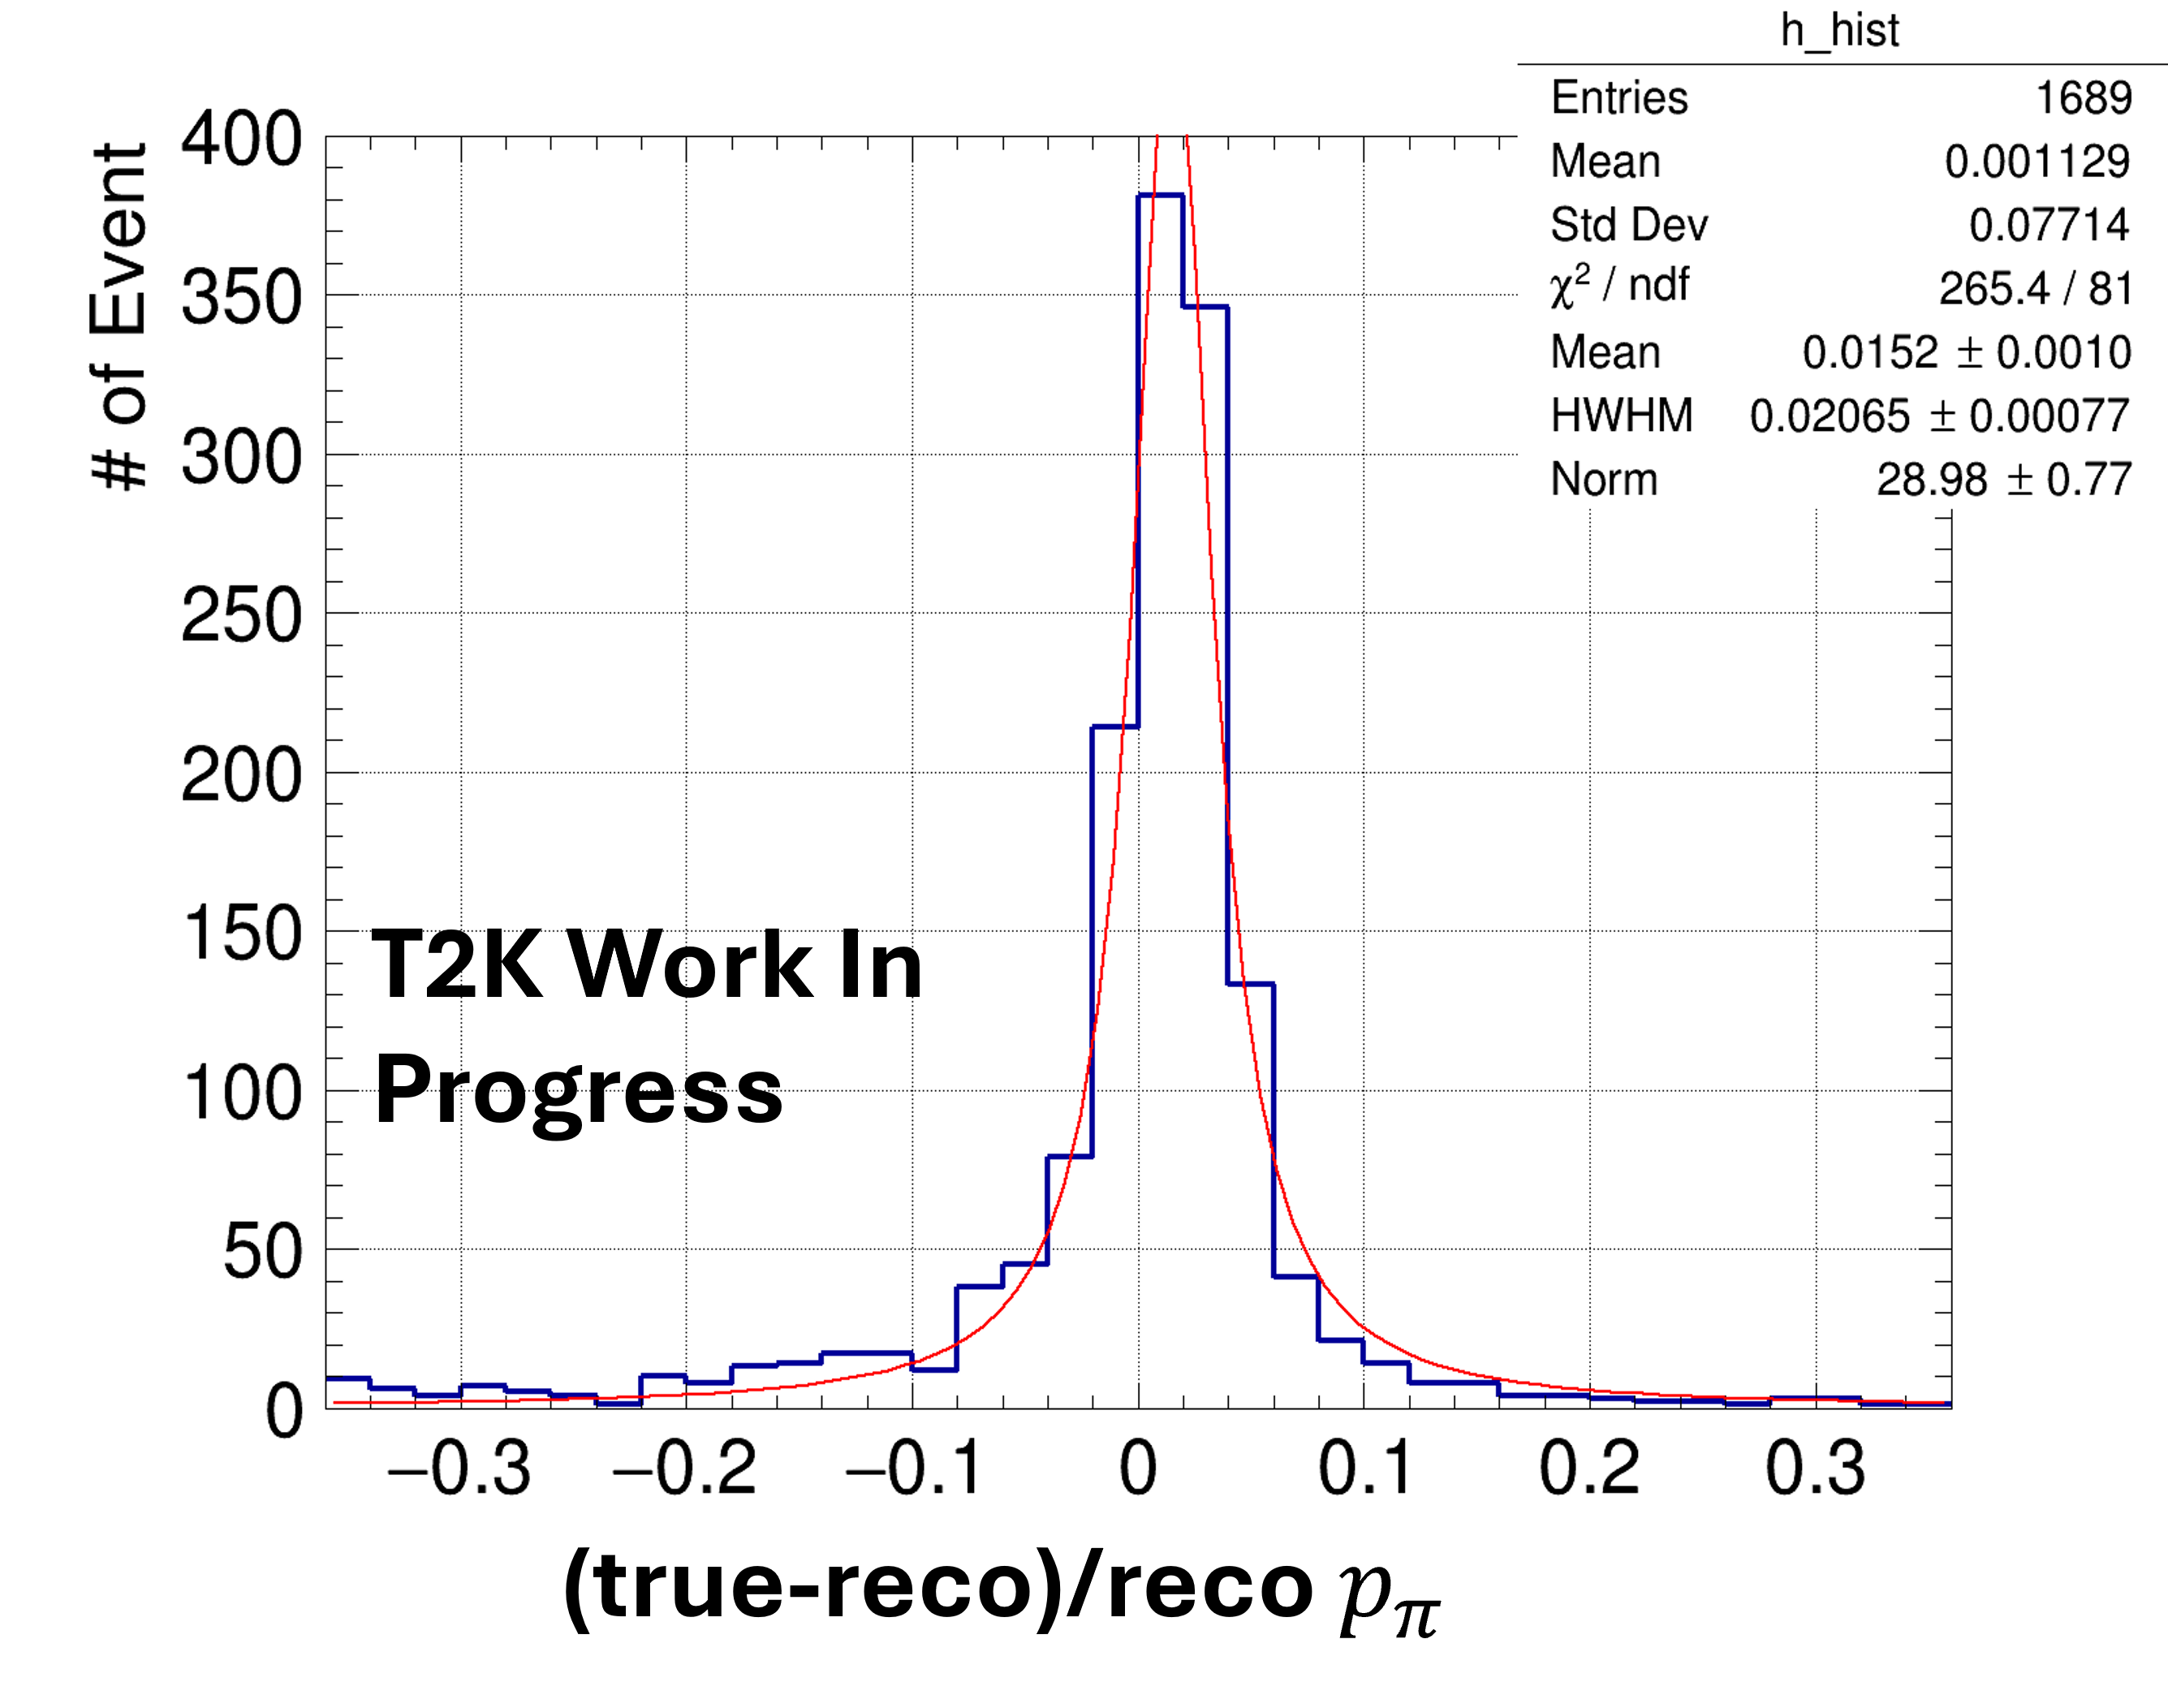
\includegraphics[width=\textwidth]{fig/ppi_res.png}
                    \caption{Momentum resolution.}
                    \label{fig:ppi-res}
               \end{subfigure}
               \begin{subfigure}{0.3\textwidth}
                    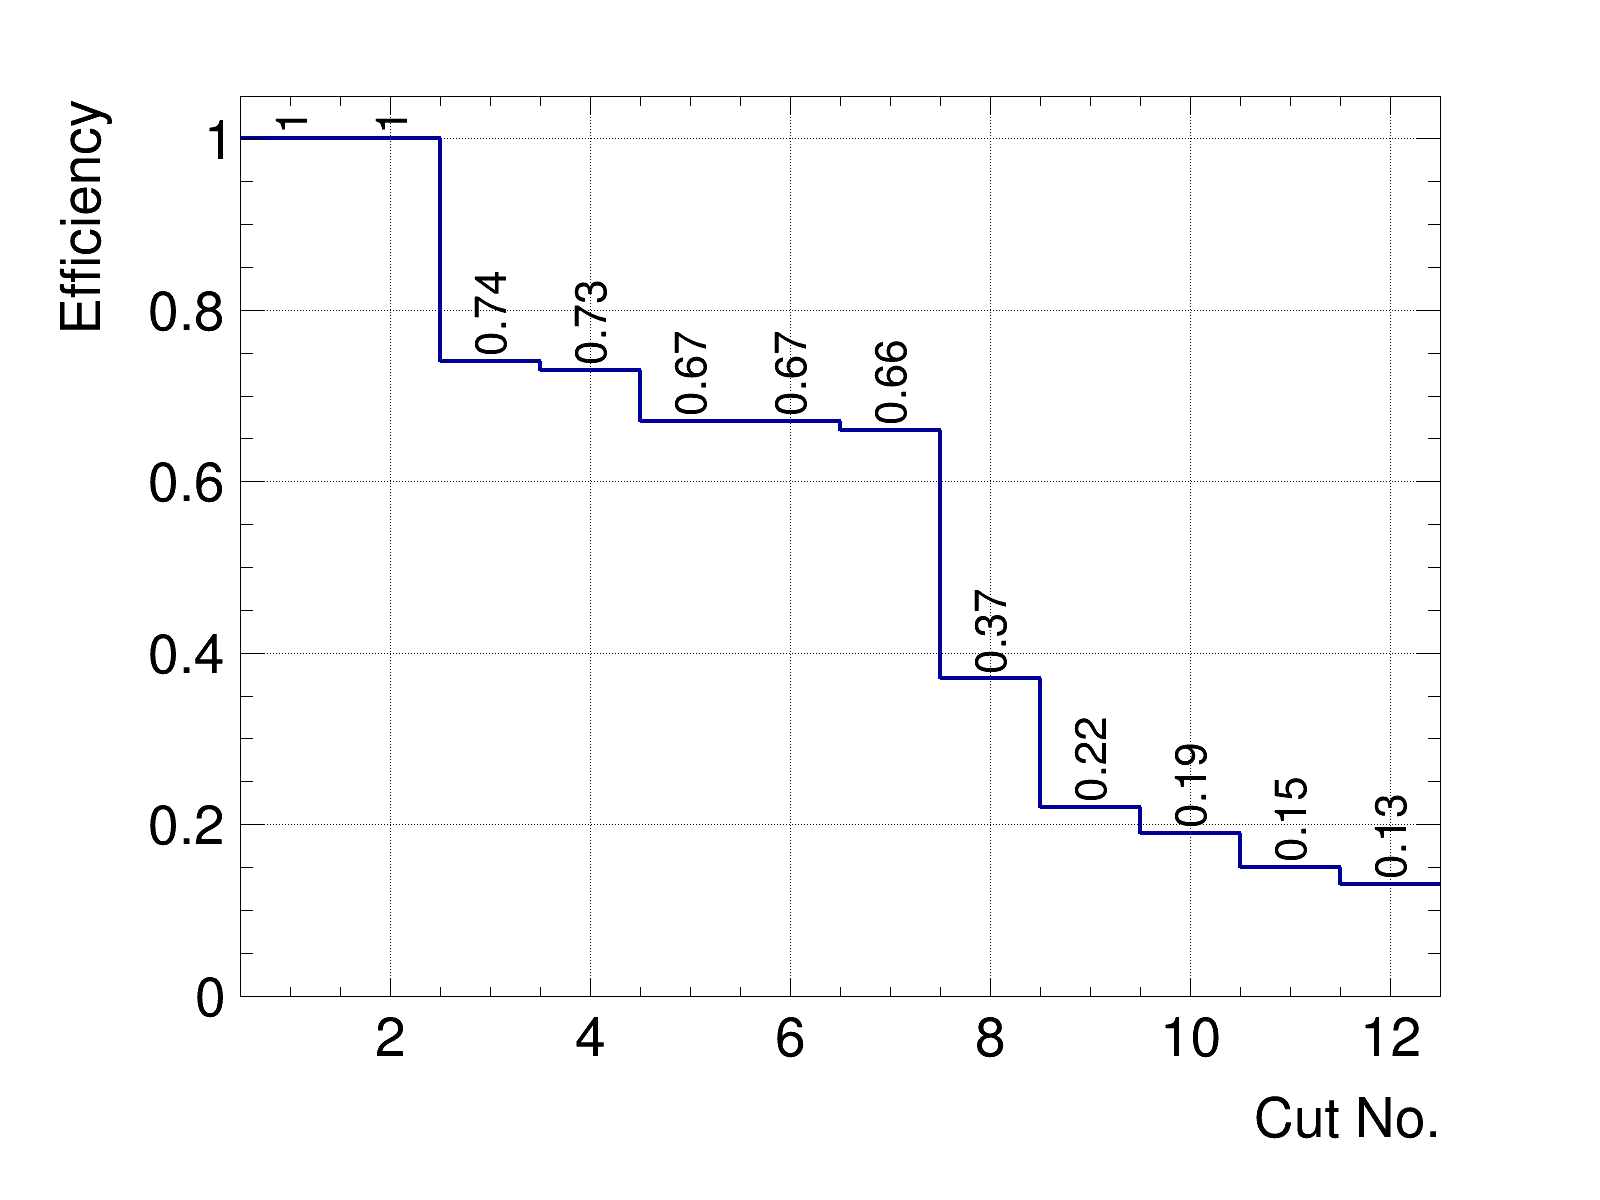
\includegraphics[width=\textwidth]{fig/INCL_p_pi_accum_eff_al11.png}
                    \caption{Accumulative efficiency.}
                    \label{fig:tl-accum-eff}
               \end{subfigure}
               \caption{Pion trackless reconstruction results.}
               \label{fig:piTLres}
            \end{figure}
            
    %------------------- ESC ----------------%
    \subsection{ESC proton selection}

         \subsubsection{Working Principles}
         Protons stopping at rest would deposit a large amount of energy, the so-called Bragg Peak, just before it stops.
         These protons tend to have their momenta better constructed as its momentum is more strongly correlated with its range. As shown in Fig.~\ref{fig:andedx2}, protons having energy below $1000$ units has large variances in momentum reconstruction. 
         \begin{figure}[h]
             \centering
             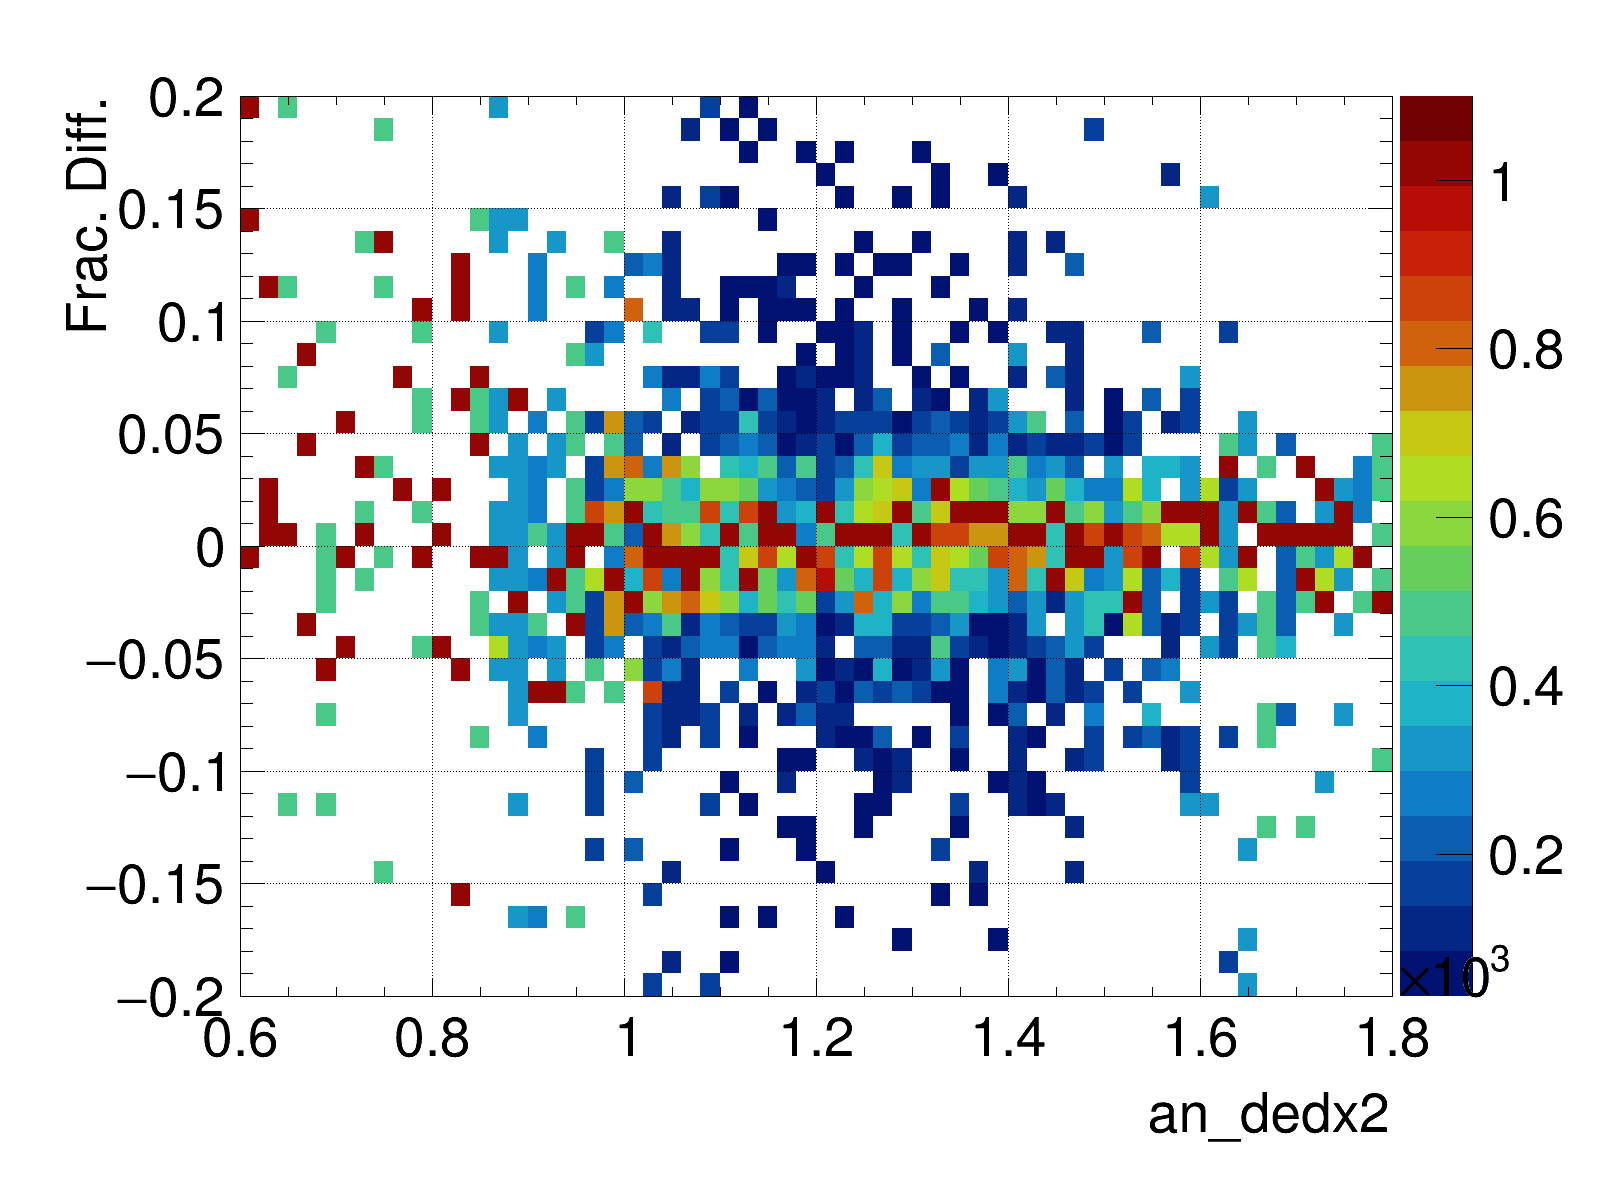
\includegraphics[width=0.5\linewidth]{fig/an_dedx2_colnor_vs_p_pr_res_hist2d_al12_zoom.png}
             \caption{Proton momentum fractional difference against energy deposited at the third last node.}
             \label{fig:andedx2}
         \end{figure}
         Hence, these protons can be selected by placing a lower boundary cut on the energy deposited at the nodes near the end of the reconstructed tracks to have a sample with a high proton momentum resolution.   
         
        \subsubsection{Implementation}
        To determine the suitable boundary values, a large particle gun proton sample is simulated and the suitable lower bounds are extracted from the resolution plots. % how many
        The lower boundary cut is implemented as an extra step on the existing $\numuccopiop$ sample, where the $p$ stands for proton.
        This selection leads to an improvement in proton momentum resolution of about $50\%$ while decreasing the efficiency by about $2/3$, as shown in Fig.~\ref{fig:pprESC-res}.   
        The drop of efficiency might seem drastic, but it proves to be necessary for the TKI analysis, as shown later in Sec.~\ref{sec:do-TKI}. The ESC selection leads to significant improvement to the TKI variables evaluation. 

        \begin{figure}[t]
           \centering
           \begin{subfigure}{0.45\textwidth}
                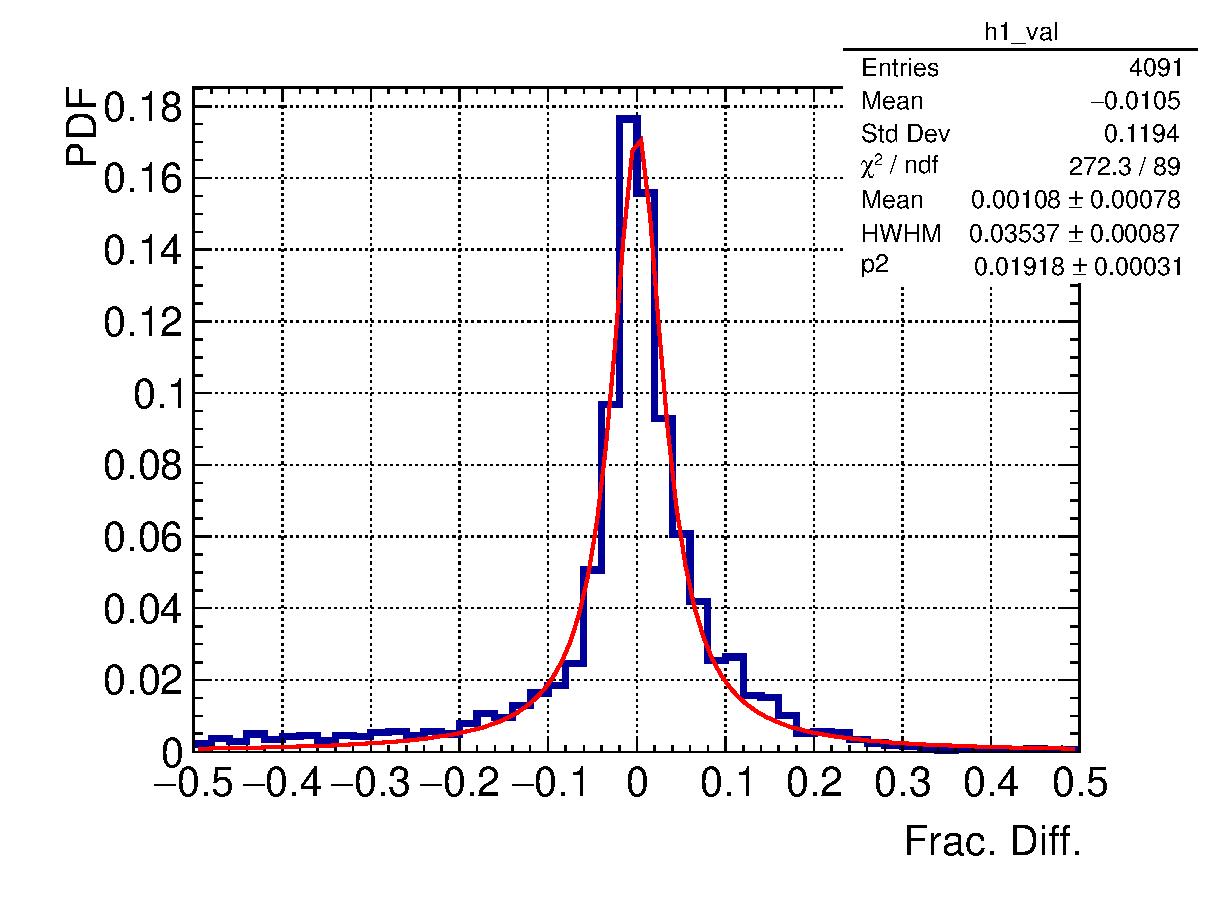
\includegraphics[width=\textwidth]{fig/p_pr_res_pdf_al13_zoom.eps}
                \caption{Momentum resolution before ESC selection.}
                \label{fig:ppr-res-bfESC}
           \end{subfigure}
           \begin{subfigure}{0.45\textwidth}
                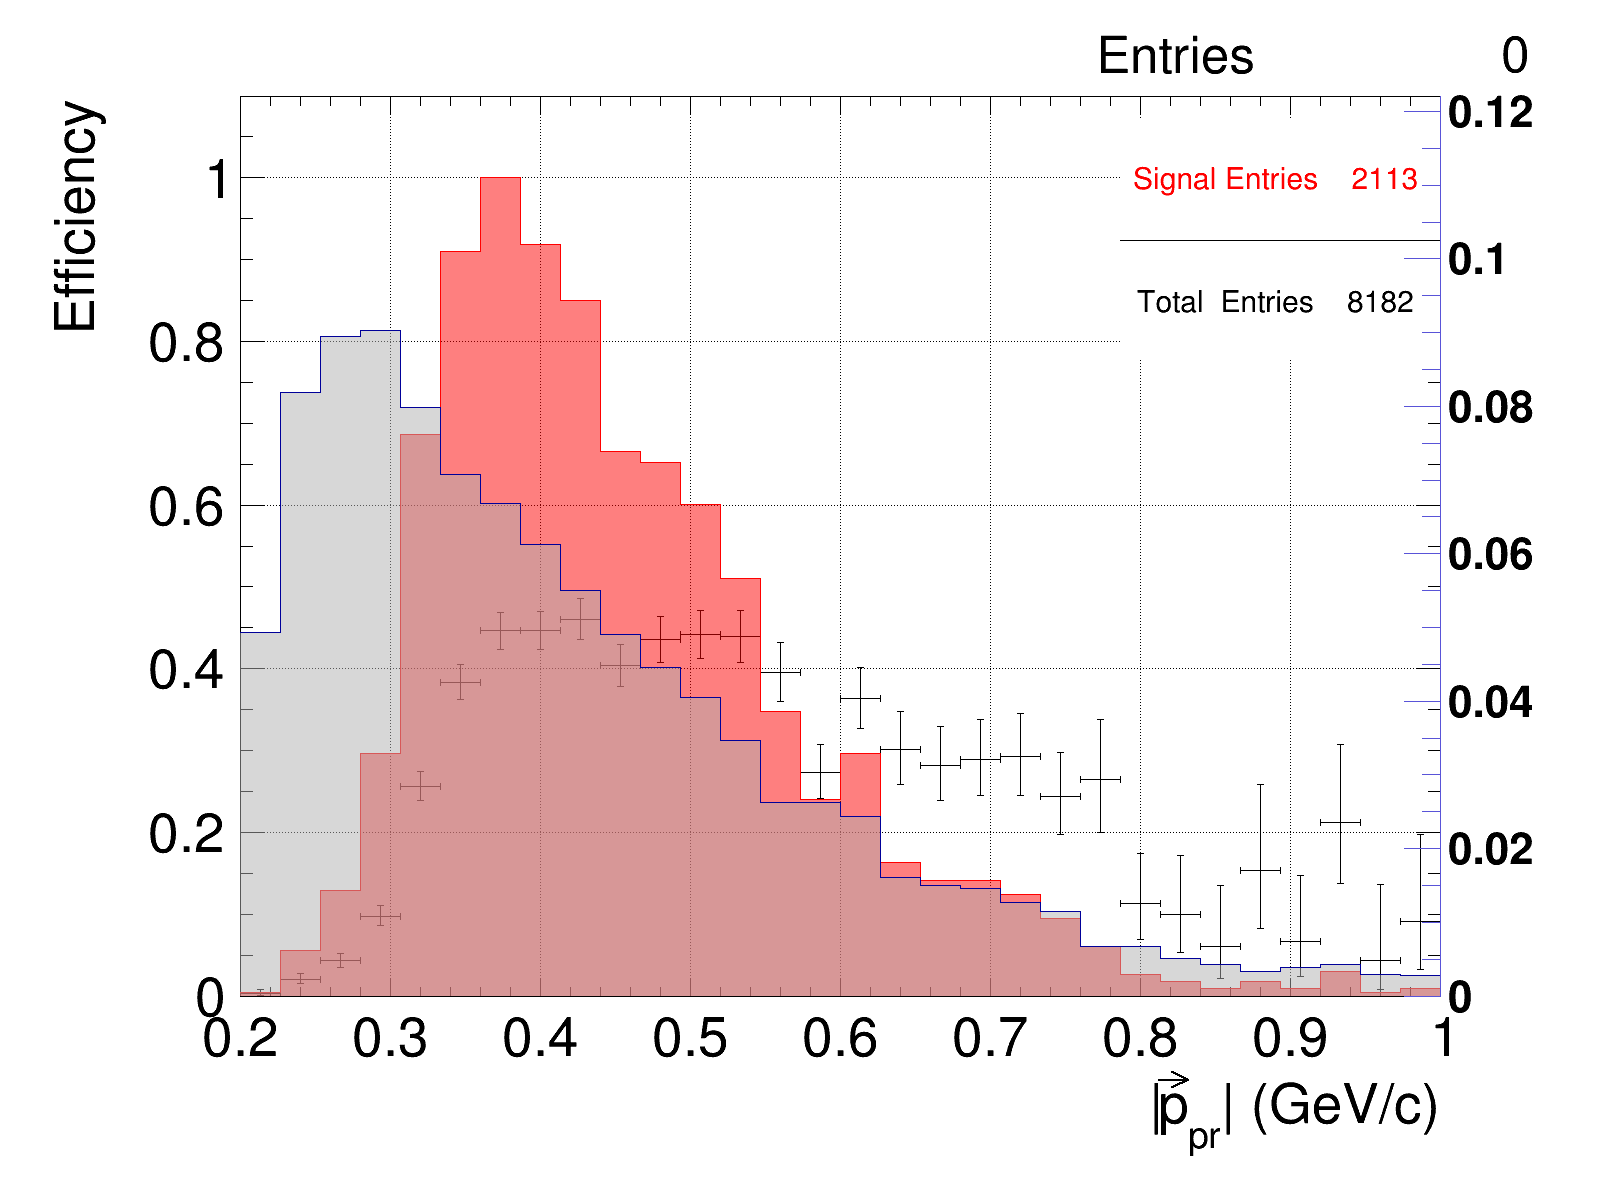
\includegraphics[width=\textwidth]{fig/p_pr_eff_al13.png}
                \caption{Selection efficiency before ESC selection.}
                \label{fig:ppr-eff-bfESC}
           \end{subfigure}
           \\
           \begin{subfigure}{0.45\textwidth}
                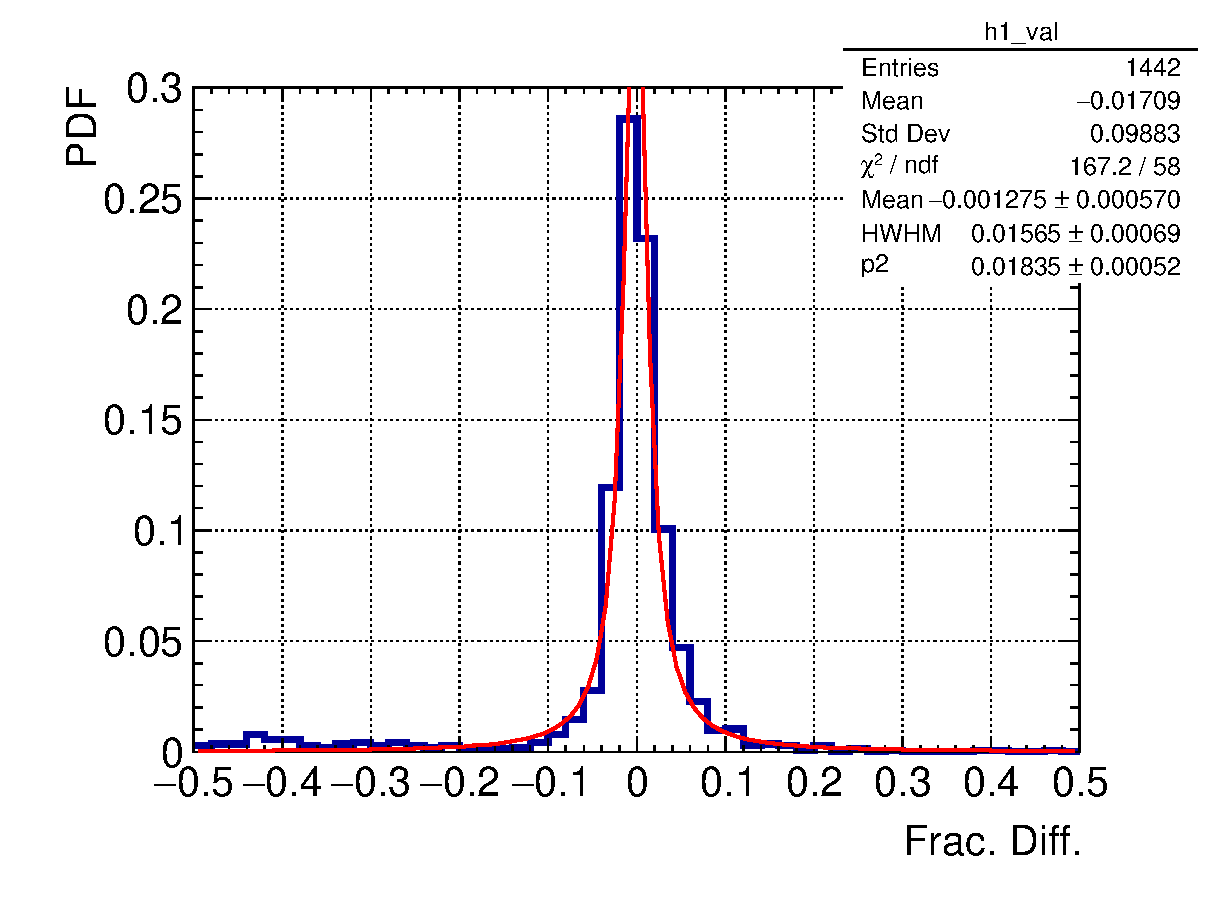
\includegraphics[width=\textwidth]{fig/p_pr_res_pdf_al14_zoom.eps}
                \caption{Momentum resolution after ESC selection.}
                \label{fig:ppr-res-afESC}
           \end{subfigure}
           \begin{subfigure}{0.45\textwidth}
                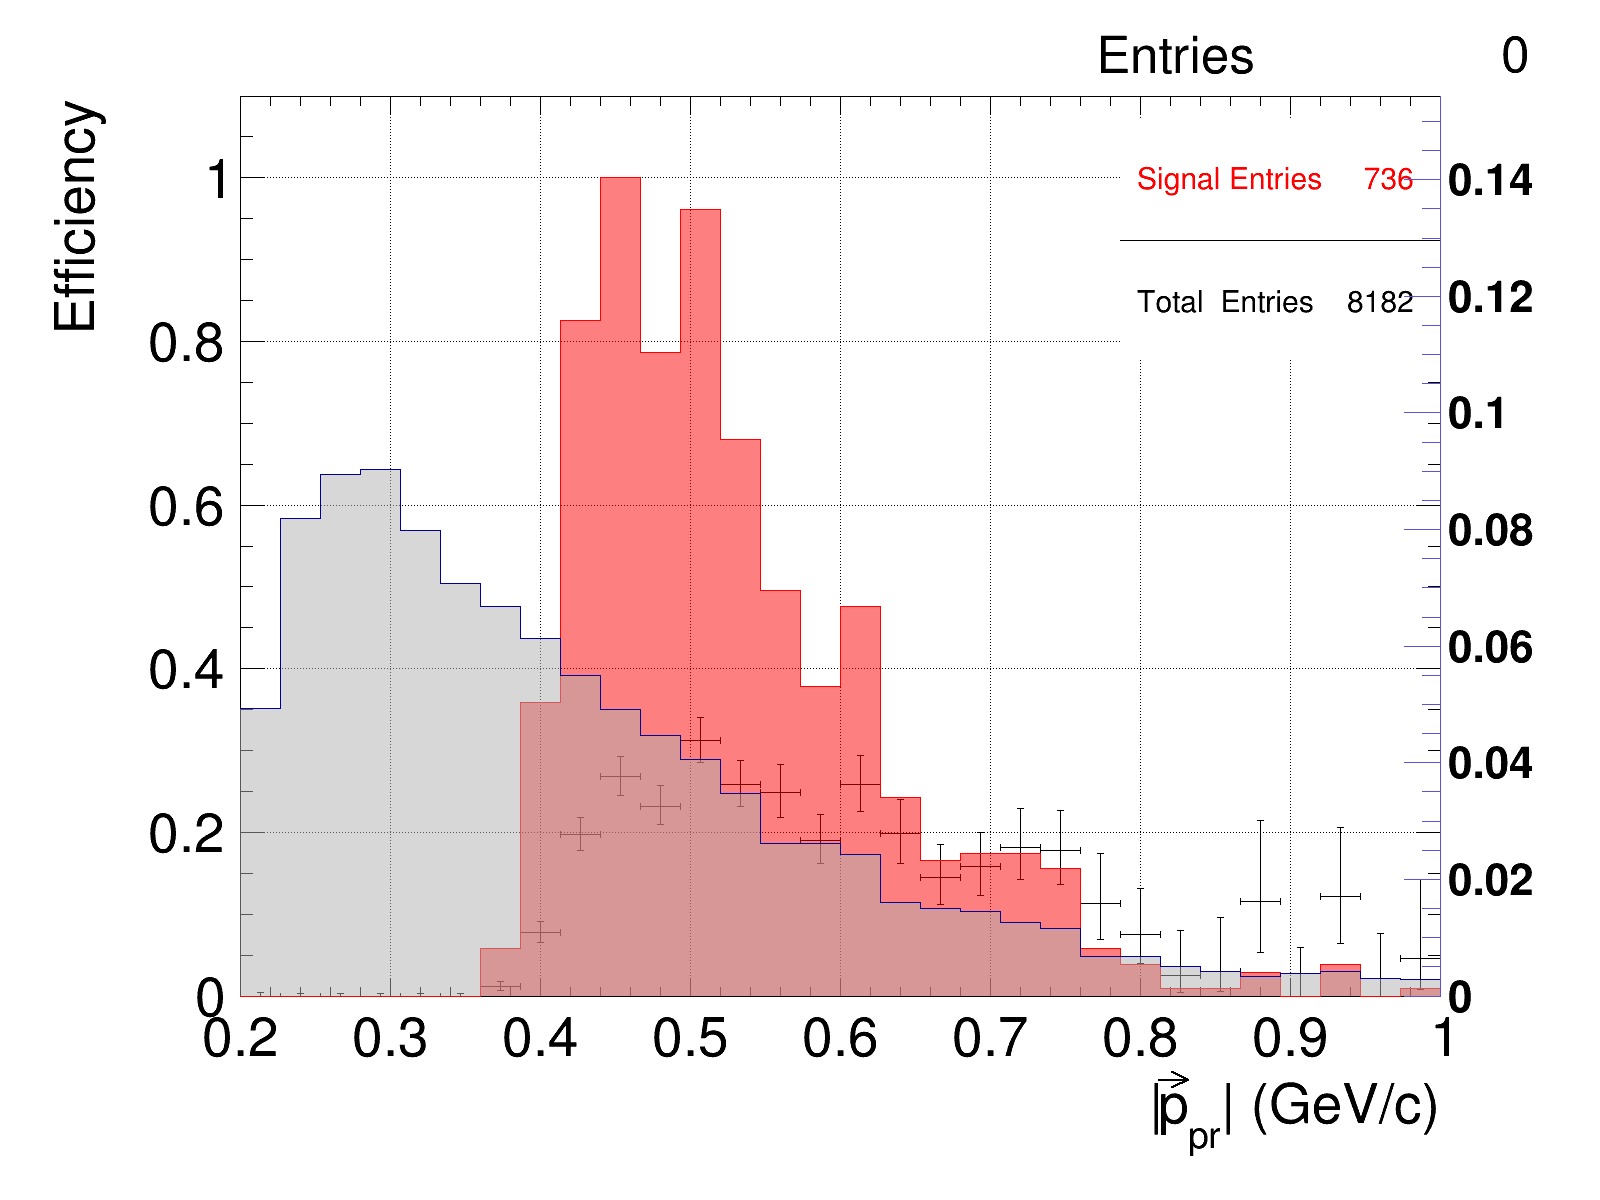
\includegraphics[width=\textwidth]{fig/p_pr_eff_al14.png}
                \caption{Selection efficiency after ESC selection.}
                \label{fig:ppr-eff-afESC}
           \end{subfigure}
           \caption{Proton ESC selection results. The grey histograms are the true probability distribution, while the pink ones are those that get reconstructed. }
           \label{fig:pprESC-res}
        \end{figure}

    

    \subsection{Discussion}
        Both the pion and ESC proton selections are finished for muons going into the vertical TPC and SFGD. The High Angle TPC reconstruction is under development and will be expected to finish in the end of July 2024. Hence, the full selection will be done in the following months. The estimation of systematic uncertainties using control samples is being developed by colleagues and is expected to be done in the next few months. 


     \subsection{systematics ovaluation}
